\section{Other Sensors}

In the previous chapters we built factor graphs with camera and IMU factors. The same framework can include any other sensor, as long as we can write its \textbf{measurement model} and the corresponding \textbf{residual}. In this chapter we see two very common cases: \textbf{GNSS}, which gives an absolute position, and \textbf{LiDAR odometry}, which gives the relative motion between two scans.

\subsection{GNSS}
\subsubsection{What is GNSS?}
\textbf{GNSS} (Global Navigation Satellite System) is the generic name for satellite-based systems that allow a receiver to estimate its \textbf{position, velocity and time} anywhere on Earth, as long as enough satellites are visible.

Examples of GNSS constellations are:
\begin{compactitemize}
    \item \textbf{GPS}, United States;
    \item \textbf{Galileo}, European Union;
    \item \textbf{GLONASS}, Russia;
    \item \textbf{BeiDou}, China.
\end{compactitemize}
A receiver can use several constellations at the same time, so that more satellites are visible.

The receiver estimates:
\begin{compactitemize}
    \item the \textbf{position} $p = [x, y, z]^T$;
    \item the \textbf{velocity} $v = [v_x, v_y, v_z]^T$;
    \item the \textbf{receiver clock offset and drift};
    \item sometimes additional states, e.g.\ the carrier-phase ambiguities.
\end{compactitemize}

\subsubsection{How does GNSS work? Satellite ranging}
GNSS is based on measuring the \textbf{distance} to several satellites:
\begin{enumerate}
    \item each satellite broadcasts a \textbf{time-tagged signal} together with its \textbf{navigation message} (orbit, clock corrections, etc.), so the receiver knows where the satellite was when it sent the signal;
    \item the receiver compares the transmit and receive times, and the difference multiplied by the speed of light $c$ gives a range called \textbf{pseudorange}:
    \[
    \rho_i \simeq c\left(t_{rx} - t_{tx,i}\right)
    \]
    \item each satellite gives one range constraint: the receiver lies on a sphere centred on the satellite. The ranges to multiple satellites intersect and constrain the receiver position.
\end{enumerate}

\begin{figure}[H]
    \centering
    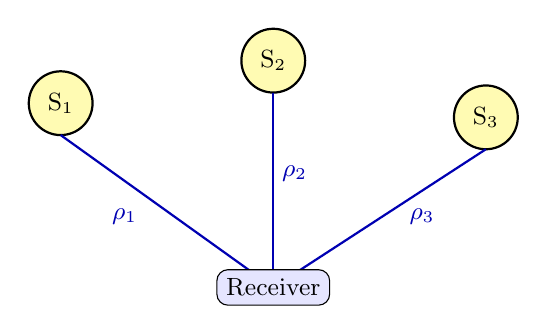
\begin{tikzpicture}[scale=0.9]
        \foreach \x/\y/\n in {-3/2.6/1, 0/3.2/2, 3/2.4/3} {
            \draw[fill=yellow!30, thick] (\x,\y) circle (0.45);
            \node[font=\small] at (\x,\y) {S$_\n$};
            \draw[thick, blue!70!black] (\x,\y-0.45) -- (0,0);
        }
        \node[draw, rounded corners, fill=blue!10, font=\small] at (0,0) {Receiver};
        \node[font=\small, blue!70!black] at (-2.1,1.0) {$\rho_1$};
        \node[font=\small, blue!70!black] at (0.3,1.6) {$\rho_2$};
        \node[font=\small, blue!70!black] at (2.1,1.0) {$\rho_3$};
    \end{tikzpicture}
    \caption{Satellite ranging: each satellite provides one range constraint}
\end{figure}

\begin{infobox}[Why ``pseudo''range?]
The satellites have very precise atomic clocks, but the receiver has a cheap clock with an unknown offset $\delta t$. Since the light travels about $300\,\mathrm{km}$ in one millisecond, even a tiny clock error gives a huge range error. The measured range is therefore not the true distance:
\[
\rho_i = \left\| p_{sat,i} - p \right\| + c\, \delta t + \text{errors}
\]
The clock offset is a fourth unknown besides $x, y, z$. This is why at least \textbf{4 satellites} are needed to compute a position, and why the receiver estimates its clock offset and drift.
\end{infobox}

\subsubsection{From geographic to local Cartesian coordinates}
GNSS provides \textbf{geographic coordinates}:
\[
p_{LLA} = \left[\, \varphi \ \ \lambda \ \ h \,\right]^T
\]
where $\varphi$ is the latitude, $\lambda$ the longitude and $h$ the ellipsoidal altitude. These angles cannot be used directly in our factor graph, which works in a Cartesian frame in metres. The conversion is done in two steps.

\textbf{1. Geodetic to ECEF.} We first convert the coordinates into the \textbf{Earth-Centered Earth-Fixed} (ECEF) Cartesian frame, whose origin is the centre of the Earth. The Earth is modeled as an ellipsoid with semi-major axis $a$ and eccentricity $e$, and $N(\varphi)$ is the radius of curvature at latitude $\varphi$:
\[
N(\varphi) = \frac{a}{\sqrt{1 - e^2 \sin^2\varphi}}
\]
\[
\begin{aligned}
X &= (N + h) \cos\varphi \cos\lambda\\
Y &= (N + h) \cos\varphi \sin\lambda\\
Z &= \left(N(1 - e^2) + h\right) \sin\varphi
\end{aligned}
\]

\textbf{2. ECEF to local ENU.} ECEF coordinates are huge numbers (millions of metres) and their axes are not aligned with the ground. We therefore define a \textbf{reference point} $(\varphi_0, \lambda_0, h_0)$, e.g.\ the starting position of the vehicle, and express everything relative to it in a local \textbf{East-North-Up} frame:
\[
p_{ENU} = R^{ENU}_{ECEF}\left(p_{ECEF} - p_{ECEF,0}\right)
\]
with:
\[
R^{ENU}_{ECEF} =
\begin{bmatrix}
-\sin\lambda_0 & \cos\lambda_0 & 0\\
-\sin\varphi_0 \cos\lambda_0 & -\sin\varphi_0 \sin\lambda_0 & \cos\varphi_0\\
\cos\varphi_0 \cos\lambda_0 & \cos\varphi_0 \sin\lambda_0 & \sin\varphi_0
\end{bmatrix}
\]
The rows of this matrix are the East, North and Up directions at the reference point, expressed in ECEF.

The resulting local coordinates are expressed in \textbf{metres}:
\[
p_{ENU} = \left[\, E \ \ N \ \ U \,\right]^T
\]
i.e.\ East, North and Up, with the reference point mapped to the origin.

\subsubsection{GNSS factor: local Cartesian position residual}
To use GNSS in the factor graph:
\begin{compactitemize}
    \item the LLA measurement is converted to the local ENU frame;
    \item the measured position $\hat p^{ENU}_{GNSS}$ is the position of the \textbf{antenna} in the world, not of the vehicle;
    \item the measurement model links the vehicle position $p^{ENU}_B$ and its rotation $R_{ENU\leftarrow B}$ to the measured antenna position, using the \textbf{antenna lever arm} $t_{B\leftarrow GNSS}$, i.e.\ the position of the antenna with respect to the vehicle.
\end{compactitemize}

\textbf{Measurement model:}
\[
\hat p^{ENU}_{GNSS} = p^{ENU}_B + R_{ENU\leftarrow B}\, t_{B\leftarrow GNSS}
\]

\textbf{Residual:}
\[
\left\| \hat p^{ENU}_{GNSS} - \left( p^{ENU}_B + R_{ENU\leftarrow B}\, t_{B\leftarrow GNSS} \right) \right\|_2^2
\]

The lever arm is important: the antenna is usually on the roof, about one or two metres away from the vehicle reference point. When the vehicle turns, the antenna moves differently from the vehicle origin, so ignoring the lever arm would give a position error of the same order. Since the residual depends on $R_{ENU\leftarrow B}$, the GNSS factor also gives some information about the \textbf{orientation} of the vehicle.

\subsection{Odometry factor}
An odometry measurement provides the \textbf{relative motion} between two consecutive poses.

\textbf{1. Measurement model.} Let $T_k \in SE(3)$ be the pose of the sensor/body at time $k$. The measured relative transformation is:
\[
Z_{k,k+1} = T_k^{-1}\, T_{k+1}
\]

\textbf{2. Residual.} The discrepancy between the predicted and the measured relative motion is computed on the \textbf{Lie algebra}:
\[
r_O = \operatorname{Log}\!\left( \hat Z_{k,k+1}^{-1}\, T_k^{-1}\, T_{k+1} \right)
\]
where $\operatorname{Log}: SE(3) \to \mathfrak{se}(3)$ maps the relative transformation error into a 6D vector (3 for the rotation and 3 for the translation). It is the inverse of the exponential map $\operatorname{Exp}(\cdot)$.

If the measurement is perfect, $\hat Z_{k,k+1}^{-1}\, T_k^{-1} T_{k+1} = I$ and its logarithm is the zero vector. As with the rotations in Section~\ref{sec:least-squares}, we cannot simply subtract two poses, because $SE(3)$ is not a vector space. So we compose them and map the error to the tangent space.

\subsection{LiDAR odometry}
\subsubsection{From scans to motion}
\textbf{LiDAR odometry} estimates the motion of the sensor by \textbf{aligning point clouds} acquired at different timestamps:
\begin{compactitemize}
    \item \textbf{input}: two point clouds $\mathcal{P}_{k-1}$ and $\mathcal{P}_k$;
    \item we estimate the rigid transformation that best aligns the two scans;
    \item \textbf{output}: the relative translation and rotation between the two acquisition times.
\end{compactitemize}
Chaining the relative poses gives a trajectory, but the errors accumulate over time (\textbf{odometric drift}).

\begin{infobox}[Important: motion distortion]
A spinning LiDAR does not acquire all its points at the same instant, but over a time interval (e.g.\ $100\,\mathrm{ms}$ for a $10\,\mathrm{Hz}$ LiDAR). If the vehicle moves during the scan, the points of the same scan are taken from different poses, and the point cloud is distorted. This motion distortion must be compensated with \textbf{deskewing}, which typically uses the IMU or an initial motion estimate to bring all the points to the same time.
\end{infobox}

\subsubsection{ICP: Iterative Closest Point}
Given a \textbf{source} cloud $\mathcal{P}_k$ and a \textbf{target} cloud $\mathcal{P}_{k-1}$, \textbf{ICP} alternates between a correspondence search and a transformation optimization:
\begin{enumerate}
    \item \textbf{initialize} the relative transformation $T^{(0)}$, e.g.\ with the identity or with an IMU prediction;
    \item \textbf{find correspondences}: for each transformed source point, find the nearest target point;
    \item \textbf{estimate the motion}: solve for the rigid transformation that minimizes the alignment error;
    \item \textbf{iterate} until convergence or until a maximum number of iterations is reached.
\end{enumerate}
The correspondences are unknown at the beginning. ICP therefore guesses them with the nearest neighbour, solves for the motion, and then improves the guess with the new transformation. For this reason a good initialization is important: if the initial guess is too far, the nearest neighbours are wrong and ICP can converge to a wrong alignment.

\begin{figure}[H]
    \centering
    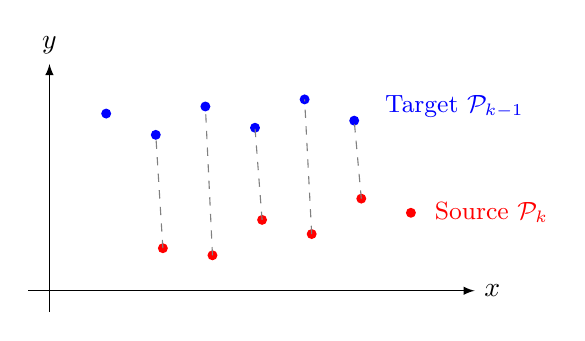
\begin{tikzpicture}[scale=0.9, >=latex]
        \draw[->] (-0.3,0) -- (6,0) node[right] {$x$};
        \draw[->] (0,-0.3) -- (0,3.2) node[above] {$y$};
        % target
        \foreach \x/\y in {0.8/2.5, 1.5/2.2, 2.2/2.6, 2.9/2.3, 3.6/2.7, 4.3/2.4} {
            \fill[blue] (\x,\y) circle (2pt);
        }
        % source (rotated and shifted)
        \foreach \x/\y in {1.6/0.6, 2.3/0.5, 3.0/1.0, 3.7/0.8, 4.4/1.3, 5.1/1.1} {
            \fill[red] (\x,\y) circle (2pt);
        }
        % correspondences
        \foreach \a/\b/\c/\d in {1.6/0.6/1.5/2.2, 2.3/0.5/2.2/2.6, 3.0/1.0/2.9/2.3, 3.7/0.8/3.6/2.7, 4.4/1.3/4.3/2.4} {
            \draw[gray, dashed] (\a,\b) -- (\c,\d);
        }
        \node[blue, font=\small, anchor=west] at (4.6,2.6) {Target $\mathcal{P}_{k-1}$};
        \node[red, font=\small, anchor=west] at (5.3,1.1) {Source $\mathcal{P}_k$};
    \end{tikzpicture}
    \caption{ICP: the source points (red) are matched to the nearest target points (blue, dashed lines) and moved to align with them}
\end{figure}

\subsubsection{ICP: alignment optimization}
Let $p^k_i$ be a point of the current scan and $q^{k-1}_i$ its corresponding point in the previous scan. The unknown transformation maps the current scan into the previous frame.

\textbf{Point-to-point ICP} solves:
\[
\hat T_{k-1,k} = \arg\min_{T \in SE(3)} \sum_{i \in \mathcal{C}} \left\| q^{k-1}_i - T\, p^k_i \right\|^2
\]
where:
\begin{compactitemize}
    \item point-to-point ICP minimizes the \textbf{Euclidean distances} between corresponding points;
    \item $\mathcal{C}$ is the set of \textbf{accepted correspondences}. Pairs that are too far apart are usually rejected as outliers.
\end{compactitemize}
This is again a nonlinear least squares problem on a manifold, which can be solved with the tools of Section~\ref{sec:least-squares} (Gauss--Newton with the $\boxplus$ update on $SE(3)$). For point-to-point ICP there is also a closed-form solution based on the SVD of the cross-covariance of the two point sets.

\subsubsection{From ICP to a factor graph odometry factor}
Let $T_k$ map coordinates from the body frame at time $k$ into the world frame. ICP estimates the relative transform:
\[
\hat Z_{k-1,k} \approx T_{k-1}^{-1}\, T_k
\]
which is exactly an odometry measurement. The odometry residual is the pose discrepancy on $SE(3)$:
\[
\boxed{r_{ICP} = \operatorname{Log}\!\left( \hat Z_{k-1,k}^{-1}\, T_{k-1}^{-1}\, T_k \right) \in \mathbb{R}^6}
\]

\begin{infobox}[What does the factor provide?]
ICP constrains the \textbf{relative pose} of two consecutive states. It does \textbf{not} provide an absolute position: a prior or another absolute sensor (e.g.\ GNSS) is needed to \textbf{anchor} the trajectory. This is the same structure as the INS factor graph of Section~\ref{sec:bundle-adjustment}: relative factors (ICP, IMU, wheel odometry) between consecutive states, and absolute factors (GNSS) on single states.
\end{infobox}
